% !TeX spellcheck = en_GB
\section{Experimental Set-up and Procedure}
\subsection{Set-Up}

\subsection{Calibration}
\subsubsection{convertion factor camera}
The strip was meassure with a calibrator at $1.2\pm 0.1\,\mathrm{mm}$ and the camara used was a Thorlabs CCD camera with dimentions of 1280x1024 pixels, each pixel with $5.2\times5.2 \mathrm{\mu m}$ according to the manufacturer.
In order to know the actual resolution of our microscope a calibration was done based on the magnification and calibration factor of the set up.
Theoritically our $C_{f}$ can be calculated as:
\\

\begin{equation}
C_{f}=\dfrac{1 px \cdot M}{d_{p}} = 1552 px/mm
\end{equation}\\
Where $M$ is the magnification and $d_{p}$ is the pixel sizes. And with a Magnification icual to the lenses used for the confocal setup is equal to the magnification $M=f2/f1=8$.
In this case the tool of Thorlab’s software was used to determine and measure the width of the microstrip. Using the equation above and the respective measumente we denote that  $C_{f} =1346 \,\mathrm{px/mm}$, with a magnification factor close to $M=7X$.


\subsubsection{Electronic components}

In order Performe our ODMR, is crucial to determine the amount of microwave power deployed into the microstrip and the diamonds. we can not have an absolut power that is been pluging into the set up. The microstrip by defoult have some transmition $T_{Ms}$ and reflecctions $R_{Ms}$ that are unkown.
For this a power coupler was added to the setup and four meassument with diferents arranges where performed as shown in the fig...
First, the power coupler was conected to the DSA in out- out possition to knoe the transmitio of it, $T_{cpl}$. on the other hand the secon setup is an Out conection to the DSA and help to determine the reflection of the CPL $R_{cpl}$. for the thirt and fouth display, the mmicrostrip was added, in the Out-Out possition ( CPL-DSA), messurion the Reflection $R_{cpl-Ms}$ and transmition $T_{cpl-Ms}$ of the hole set.

\begin{figure}
	\centering
	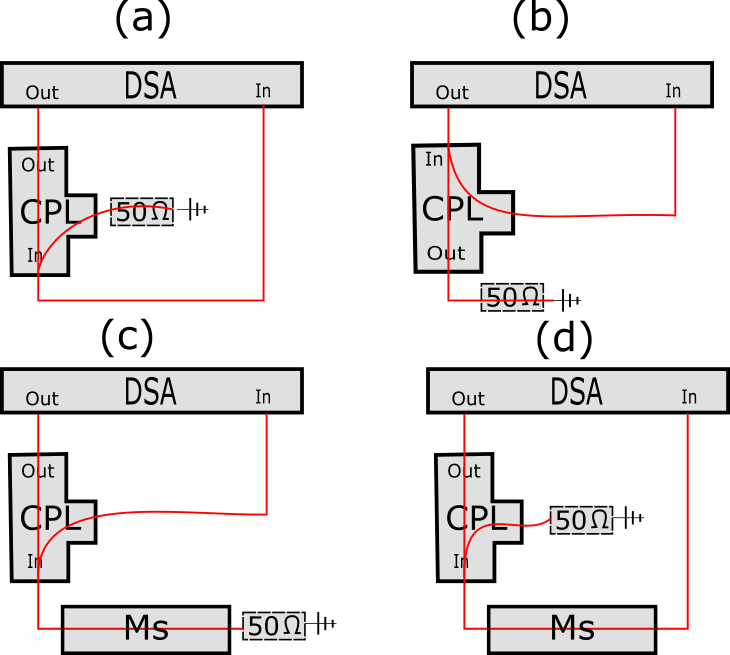
\includegraphics[width=0.7\linewidth]{../figures/APD}
	\caption[diferent arranges of the CPL and MicroStrip conected to the DSA]{(A) CPL conected to the DSA in Out-Out direction messuring $T_{cpl}$, (b) Cpl conected in Out-In secuence and meassuring $R_{cpl}$, (c) CPl and microstrip conected in Out-Out mode and measuring the $R_{cpl-Ms}$ (d) CPL and Microstrip conected in Out-Out moded and meassuring $T_{cpl-Ms}$}
	\label{fig:apd}
\end{figure}

The DSA was set at 0 Dbm and a sweep centered at 2.8GHz frequancy. A 50$\Omega$ resistance was used for the losses ends as shown. The next figure display the four signals of the diferent arranges.
\begin{figure}
	\centering
	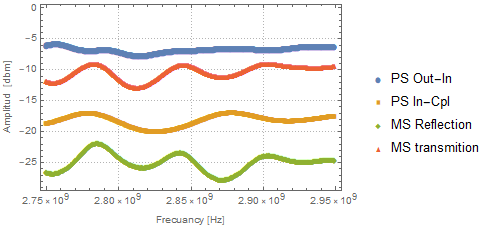
\includegraphics[width=0.7\linewidth]{../figures/microstrip}
	\caption{Atenuattion od the power at 0dBm from top to bottom: $T_{CPL}$,$T_{Cpl-Ms}$, $R_{CPL}$ and $R_{Cpl-MS}$}
	\label{fig:microstrip}
	\end{figure}

The total transmition and reflection ws simply calculated by a sustraction of the Ms trasmition in the diferent processes as next.

\begin{align}
T_{Ms}&=T_{cpl-Ms}-T_{cpl}\\
R_{MS}&=R_{cpl-Ms}+T_{cpl}-R_{cpl}
\end{align}


The attenuation in this cases for the transmission remains close to cero, specially in the center of the sweep while the reflection as shown reduces drasticly. This gives  us the facts that the power transmitted is close to the 0dBm used in the DSA and few of it is been reflected.

\begin{figure}
	\centering
	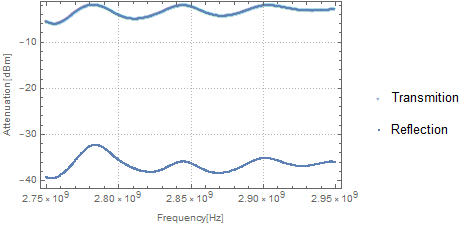
\includegraphics[width=0.7\linewidth]{../figures/microstrip-trasm-eflect}
	\caption[trans-refl]{Ateniation of the resultant transmition (top) and reflectrion (bottom) at the Micristrip, at 0dBm in a 2.8GHZ frequency center.}
	\label{fig:microstrip-trasm-eflect}
\end{figure}







\subsection{Measurements}